%%%%%%%%%%%%%%%%%%%%%%%%%%%%%%%%%%%%%%%%%%%%%%%%%%%%%%%%%%%%%%%%%%%%%%%%%%%%%%%%%%%%%
%%%%%%%%%%%%% DFS and BFS
%%%%%%%%%%%%%%%%%%%%%%%%%%%%%%%%%%%%%%%%%%%%%%%%%%%%%%%%%%%%%%%%%%%%%%%%%%%%%%%%%%%%%%%%%
\documentclass[../main.tex]{subfiles}
\begin{document}

% The basic breath-first and depth-first search we learned in Chapter~\ref{chapter_non_linear_graph} is like a linear search on linear data structures. There are more advanced universal graph search techniques: 
% \begin{enumerate}

    
%     \item Better Efficiency: 
%     \begin{enumerate}
%         \item Bidirectional Search that can  increase the efficiency of the BFS shown in Section~\ref{}.
%         \item Application of DFS on Problem Searching Space: Backtracking techniques to prune the searching space based on DFS in Section~\ref{sec_backtrack}. 
%     \end{enumerate}
% \end{enumerate}

% \subsection{Implementation}



% A mutant for trees to visit it level by level
% \begin{lstlisting}[language = Python]
% def BFS(root):
%     q = [root]
%     root.visited = 1
%     level = 0
%     while q:
%         n=q.pop()
%         visit(n) #finish visit
%         for node in n.adjacent:
%             if not node.visited:
%                 node.visited = 1 #start to visit 
%                 q.insert(0,node)
% \end{lstlisting}
%%%%%%%%%%%%%%%%%%%%%%Bidirectional%%%%%%%%%%%%%%%%%%%%%%%%

%\subsection{$A^*$}





% \section{Backtracking}% for Constraint Satisfaction Problem}
% \label{sec_backtrack}
% ``A  variant  of  Depth  First  Search  is  called  Back  Tracking search, which uses less memory. In this search only one successor  is  generated  at  a  time  rather  than  all successors. Each partially expanded node remembers which successor to generate  next.  In  this  way  only  $O(m)$  memory  is  needed rather  than  $O(b^m)$.  It  is  the  most  common  algorithm  for solving constraint satisfaction problem (CSP)." (Searching and Optimization Techniques in Artificial Intelligence: A Comparative Study $\&$ 
% Complexity Analysis)



\paragraph{Visualize Backtracking} Let us represent different $s$ as a node in a tree. Initial state $s=[]$ as the root node. The first level represents all possible states for $s=(s_0)$ of length 1, and the second level for $s=(s_0, s_1)$ of length 2. And the edge represents making a choice out of all items in the ordered set $A$. If we reach to end condition (leaf candidates) we succeed and the search stop. If the partial candidate can not satisfy the constraint, we return to the root node, and reset the state ('backtrack'). The process is shown in Fig.~\ref{fig:backtrack_tree}. 
\begin{figure}[h!]
    \centering
    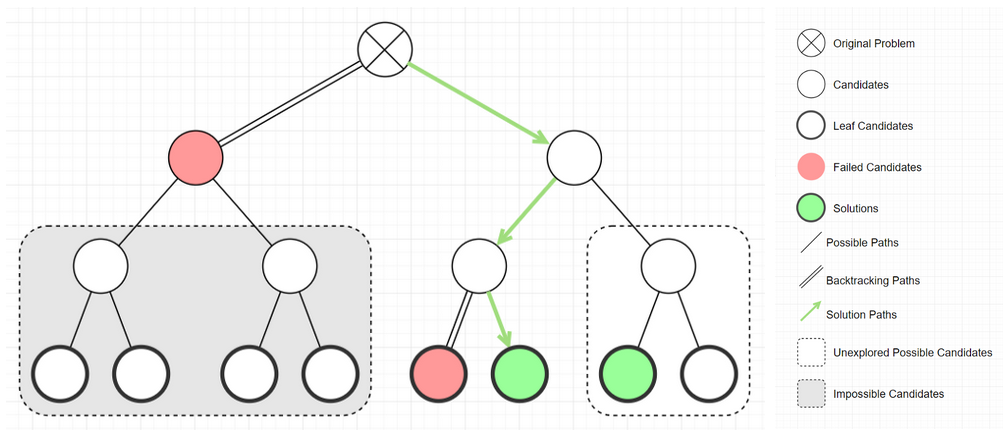
\includegraphics[width=0.98\columnwidth]{fig/back_tree_possibility.png}
    \caption{Tree of possibilities for a typical backtracking algorithm}
    \label{fig:backtrack_tree}
\end{figure}

\paragraph{Backtrack Template} We list the template here which we summarized after viewing different backtracking algorithms. It usually is composed of two parts: initialization and main dfs backtracking. After we figure out our state vector $s$ where in our template is \texttt{state\_tracker} with total search tree depth $n$. In the main backtracking state: we first generate candidates according to previous states and then try out each candidate by iteration. We set the state before call recursive function to the next depth and reset the state after we return and move on to try next candidate.  
\begin{lstlisting}[language=Python]
def backtrack():
  # initialization
  A #a working data structure, either a list of candidates or a graph or a matrix representing a board
  state_tracker = []*n
  assist_state_tracker
  # main backtracking
  def dfs(d, n):
    '''d: depth representing level in the tree'''
    if d == n:
      return
    candidates = generate_candidates(state_tracker, assist_state_tracker)
    for c in candidates: 
      set_state(state_tracker, assist_state_tracker, c)
      dfs(d+1, n)
      reset_state(state_tracler, assist_state_tracker, c)
      
  dfs(0, n)
\end{lstlisting}

\paragraph{Complexity Analysis} The time complexity of backtracking can be obtained from analyzing the search tree. The worst case incurs when the complete result occurs at the right most of the search tree, thus we need to traverse all the paths resulting visiting each node twice-one forward and one backward. Assume the cost to generate and visit a node is $O(2)$, and the total time complexity will be $O(|V|)$, where $|V|$ is the total nodes in the traverse tree. 






In this chapter, the organization is as follows:
\begin{enumerate}
    \item Show Property 1: We will first show how backtrack construct the complete solution incrementally and how it backtracks to its previous state in Sec.~\ref{sec_enumeration}. 
    \begin{enumerate}
        \item \textbf{On Implicit Graph:} start with the combination and permutation problem to show us how the backtracking works in Section~\ref{backtrack_permutation} and ~\ref{sec_combination} with simple and commonly seen combinatorial problems: combination and permutation.
        \item \textbf{On Explicit Graph:} Enumerating all paths between the source and target vertex in a graph drawing in Section~\ref{subsec_all_paths}. Similarly, it can be applied on enumerate all spanning trees, graph partition.   
        \end{enumerate}
    \item  Show  Property 2: we demonstrate the application of search pruning in backtracking through CSP problems in Section~\ref{sec_sudoku}.
\end{enumerate}
%%%%%%%%%%%%%%%%%%%%Combination%%%%%%%%%%%%%%%%%%%%%%%%%%%
\section{Enumeration}
\label{sec_enumeration}
\subsection{Permutation}
\label{backtrack_permutation}


\paragraph{Implicit Graph} In the graph, each node is either a partial or final solution. If we look it as a tree, the internal node is a partial solution and all leaves are final solutions. One edge represents generating the next solution based on the current solution. The vertices and edges are not given by an explicitly defined graph or trees, the vertices are generated on the fly and the edges are implicit relation between these nodes. 

\paragraph{Backtracking VS DFS} The implementation of the state transfer we can use either BFS or DFS on the implicit vertices.  With recursive DFS, we can start from node [], and traverse to [1,2], then [1,2,3]. Then we backtrack to [1,2], backtrack to [1], and go to [1, 3], to [1, 3, 2].  To clear the relation between backtracking and DFS, we can say backtracking is a complete search technique which systematically builds the search tree (implicitly and not graph) and DFS is an ideal way to implement it. 


\paragraph{Back to Permutation}
We can generalize Permutation, Permutations refer to the permutation of $n$ things taken $k$ at a time without repetition, the math formula is $A_{n}^{k} = n *(n-1)*(n-2)*...*k$. In Fig.~\ref{fig:backtrack_permutation}, we can see from each level $k$ shows all the solution of $A_{n}^{k}$. The generation of  $A_{n}^{k}$ is shown in the following Python Code.%Compared with combination,  [a, b] and [b, a] would be considered as different solution. The relation of the number of combination and permutation solution can be described in formula: $C_{n}^{k}=\frac{A_{n}^{k}}{k!}$, where $k!=k*(k-1)...*1$. So $A\ge C$.





% (N-Queens :  
% permutations
%  with backtracking
% Soduko     :  
% counting
%  with backtracking
% Scheduling:  
% subsets
%  with backtracking\url{https://www.cs.princeton.edu/~rs/AlgsDS07/24CombinatorialSearch.pdf})
 






 % Also, in this process, we can trim the branches, so actually backtracking is DFS with trimming and backtrack to the previous stages. 


\subsection{Combination}
\label{sec_combination}



Note: To generate the power set, backtracking is NOT the only solution, if you are interested right now, check out Section~\ref{part4_array_combine}.





% \subsection{Analysis}
% % \paragraph{Backtracking VS DFS} The implementation of Backtracking is equivalent to a DFS on the implicit or explicit search space and visiting each vertex no more than once.  Backtracking is a technique to build up solution spaces incrementally and each exactly only once. And once one path reaches to the end, it backtrack to its previous state and try another candidate. DFS is a natural way to implement backtarck technique. 





% \paragraph{Applications} Backtracking can be applied where we can incrementally build up our final soultion from partial solution. It is a searching technique that applied on implicit graph which is built on-the-fly. It guarentees that it only visit each search vertex no more than once. The problems that backtracking can be used are these three types: (1) Combinations (Section~\ref{sec_combination}), (2) Permutations (Section~\ref{sec_permutation}), (3) enumerate all paths from a to b in graph. and (3) Optimization problems with constraints such as classical travels salesman, puzzles, and sudoku (Section~\ref{sec_sudoku}). In the first three cases, backtracking visit each implicit or explicit vertex exactly once in the searching space. And for problems with restraints, we can do search pruning and we end up amortizely visiting each vertex less than once which is more efficient compared with an exhaustive graph search such as DFS and BFS. 

\section{Solve CSP with Search Prunning}
\label{sec_sudoku}


\end{document}